\documentclass[11pt]{article}
\usepackage[margin=1in]{geometry}
\usepackage[T1]{fontenc}
\usepackage{lmodern}
\usepackage{booktabs}
\usepackage{amsmath}
\usepackage{graphicx}
\usepackage{xcolor}
\usepackage{tikz}
\usepackage[hidelinks]{hyperref}
\usepackage{listings}
\lstset{basicstyle=\ttfamily\footnotesize,columns=fullflexible,frame=single,breaklines=true}

\title{Code Mode for Governed Enterprise CRM Access:\\
An Empirical Comparison of Sandboxed Program Execution and Per-Call Tool Use over Salesforce}
\author{Srinivasa Pusuluri\\[2pt]\small \url{https://www.linkedin.com/in/pusulurisrinivasa/}}
\date{November 2026}

\begin{document}
\maketitle

\begin{abstract}
Large language model (LLM) agents usually access enterprise systems through one tool call per operation, with every intermediate result passing through the model's context. \emph{Code Mode} replaces this pattern: the model writes a single program against typed APIs, and the program runs in an isolated sandbox that calls the tools on the model's behalf. We present an open implementation of Code Mode for Salesforce, exposed to Claude through the Model Context Protocol (MCP), together with a host-side governance layer: per-user OAuth, role-based access control, field-level security, human approval for writes, redaction, and a hash-chained audit log. We compare Code Mode with a deliberately strong per-call baseline on five identical CRM workflows (30 runs each) and run the platform against a live Salesforce Developer Edition org. Measured results: Code Mode reduced model round trips by 33--50\% and tool invocations by 67--94\%, with identical Salesforce API consumption and 100\% task success in both modes. Estimated results: input tokens fell by 7.5--35.1\% when API type declarations were preloaded, but \emph{rose} by 11--57\% when the model also had to call a discovery tool, and output tokens rose by 44--86\% on four of the five workflows because generating a program costs more than emitting a short tool call. Under a stated latency model, Code Mode was slower end to end on four of five small workflows and 18\% faster only on the fan-out workflow. We also report two defects that only the evaluation exposed: lost audit events under parallel tool calls, and a synchronous infinite loop that stalled the shared gateway despite a configured CPU limit. We extend the platform with prompt-injection guardrail policies at the same checkpoint, including a taint rule that refuses writes after an execution has read injected text, and with OpenTelemetry tracing. We then evaluate tools, agent trajectories, retrieval-augmented answers and guardrails over ten repeated runs. All four suites were stable across runs. The detector reached precision 1.0 and recall 1.0 on in-distribution attacks, but caught only 3 of 6 held-out paraphrases. All nine end-to-end attack scenarios were contained, and guardrails added a median of 0.2--2.1\,ms per execution. We conclude that Code Mode's clearest benefits are fewer round trips and tool calls, and that token and latency savings depend on fan-out, payload size and how types are delivered.
\end{abstract}

\section{Introduction}
Agents that read and write CRM data are a common enterprise use of LLMs. The prevailing integration pattern exposes each operation (search accounts, list cases, create a case) as a separate tool. A task that needs ten lookups then needs several model turns, and each raw record returned by a tool is read by the model.

Code Mode, popularised by Cloudflare~\cite{cfcodemode} and discussed by Anthropic as code execution with MCP~\cite{anthropiccodeexec}, inverts this. The model is shown TypeScript declarations for the available operations and writes one program; the program runs in a sandbox and returns a compact result. The idea is related to executable code actions for agents~\cite{codeact}, but brings a new constraint in enterprise settings: generated code is untrusted, while the data it touches is governed by access controls that must still hold.

This paper makes five contributions:
\begin{enumerate}
\item An open implementation of a Code Mode gateway for Salesforce, built on Cloudflare Dynamic Workers and MCP, with a single host-side checkpoint through which every sandbox call passes (Section~\ref{sec:design}).
\item A controlled comparison against a strong per-call baseline on five workflows, separating \emph{measured} quantities (round trips, tool calls, API calls, gateway latency, success) from \emph{estimated} ones (tokens, model time) (Sections~\ref{sec:method}--\ref{sec:results}).
\item A live-org check that the same programs run unchanged against a real Salesforce org under user-scoped OAuth.
\item Prompt-injection guardrail policies enforced at the checkpoint, OpenTelemetry tracing, and a repeatable evaluation of tools, agent trajectories, retrieval and guardrails (Sections~\ref{sec:guard} and~\ref{sec:quality}).
\item Failure findings and the mitigations we applied, which we believe generalise to other Code Mode deployments (Section~\ref{sec:findings}).
\end{enumerate}

\section{Background}
\paragraph{Tool use.} ReAct~\cite{react} interleaves reasoning and actions; Toolformer~\cite{toolformer} trains models to call APIs. In both, each action is a separate model decision.
\paragraph{Code as action.} CodeAct~\cite{codeact} shows that letting agents emit executable Python can raise success rates and reduce the number of turns compared with JSON tool calls.
\paragraph{MCP.} The Model Context Protocol~\cite{mcp} standardises how clients discover and call tools on remote servers. Code Mode can be offered over MCP by exposing a small number of meta-tools instead of one tool per operation.

\section{System design}\label{sec:design}
\paragraph{Interface.} The gateway exposes two MCP tools. \texttt{discover\_capabilities} returns, for the authenticated user only, TypeScript declarations of the 29 registered operations they may call (sales, service, CPQ, metadata, Data Cloud, Agentforce, and a second system, NetSuite). \texttt{execute\_code} accepts one TypeScript program.
\paragraph{Execution.} Programs are type-stripped, parsed, statically screened, and run in a fresh Cloudflare Dynamic Worker isolate with outbound network disabled and no credentials or environment bindings. Tests use a QuickJS WebAssembly isolate implementing the same executor interface.
\paragraph{Single checkpoint.} Each \texttt{sf.*} call inside the sandbox is a remote procedure call to the host. One function performs, in order: role-based authorisation and allowlisting; per-user rate limits and per-execution call budgets; schema validation with Zod; a human-approval gate for writes; field-level-security filtering using the user's own object describe; query construction from validated identifiers and escaped literals (no raw query path exists); redaction of sensitive values; and an append to a hash-chained audit log.
\paragraph{Identity.} Each Claude user authorises their own Salesforce account through OAuth 2.0 with PKCE. Tokens are encrypted at rest with AES-256-GCM. Salesforce therefore enforces that user's object permissions, field permissions and sharing rules; the gateway never acts as a shared integration user.
\paragraph{Writes.} A write first returns \texttt{approval\_required}. A different user approves the exact tool, arguments and requester (bound by a hash). Re-running the program consumes the approval once; any change to the arguments requires a new approval.

\subsection{Prompt-injection guardrails}\label{sec:guard}
Text inside CRM records is attacker-controllable: anyone who can file a case, send an email-to-case or edit a Knowledge article can plant instructions that the model later reads. This is indirect prompt injection~\cite{greshake,owasp}. The checkpoint therefore scans every string in every tool result, and the final program result, before it reaches the sandbox or the model. Policies have five parts:
\begin{enumerate}
\item \emph{Detection.} Pattern rules in ten categories: instruction override, role hijack, fake system or turn markup, tool coercion, secret seeking, exfiltration links (for example markdown images with query strings), hidden Unicode (zero-width, bidirectional and tag characters), active HTML, untrusted links and encoded payloads.
\item \emph{Action per category.} \texttt{allow}, \texttt{flag}, \texttt{sanitize} (neutralise the matched span and keep the rest of the field), \texttt{quarantine} (replace the field) or \texttt{block} (fail the call). A monitor mode reports without changing anything.
\item \emph{Taint.} Once an execution has read text at or above a severity threshold, every write in that execution is refused before an approval is requested. This follows the information-flow idea of separating untrusted data from privileged actions~\cite{camel}: even if the model is fooled, the planted text cannot cause a write in the same run.
\item \emph{Write inputs} that carry injection text are refused, so planted text is not persisted back into the org.
\item \emph{Reporting}: findings go into the execution metadata (with a notice telling the model to treat record text as data), the audit chain and trace events.
\end{enumerate}
Live mode refuses to start with guardrails disabled. Approvals, the network-less sandbox and least-privilege capabilities still hold when detection fails.

\subsection{Observability}
Each execution is exported as an OpenTelemetry trace over OTLP: one \texttt{execute\_code} span with a child span per tool call. The spans are annotated with the OpenTelemetry GenAI semantic conventions~\cite{otelgenai} and OpenInference span kinds~\cite{openinference}, so open-source backends (Phoenix, Langfuse, Jaeger, Tempo) can display them. A W3C \texttt{traceparent} from the agent links the agent's and the gateway's traces. Spans carry metadata only by default. Capturing code and results is opt-in and refused in live mode.

\section{Method}\label{sec:method}
\paragraph{Workflows.} Five CRM tasks with different shapes: \emph{Account 360} (search, then three parallel reads), \emph{Sales pipeline} (accounts, then aggregate and list opportunities), \emph{Customer risk} (accounts with custom fields, open cases, opportunity trends), \emph{Service intelligence} (three dependent pages of cases), and \emph{Cross-system analysis} (eight accounts, each joined with two NetSuite calls).
\paragraph{Data.} A deterministic mock Salesforce org (8 accounts, 14 contacts, 16 opportunities, 14 cases) that simulates per-user CRUD, field-level security and sharing.
\paragraph{Approaches.}
(1)~\emph{Traditional MCP}: each operation is a separate tool. We give this baseline every advantage: all independent calls in a turn are issued in parallel, and object metadata is cached across calls.
(2)~\emph{Code Mode, discover + execute}: the model calls \texttt{discover\_capabilities}, then \texttt{execute\_code}.
(3)~\emph{Code Mode, execute only}: type declarations are preloaded in the model's context (for example via a project instructions file), so only \texttt{execute\_code} is called.
All three run against the same gateway, the same user and the same policies. Code Mode programs are the hand-written reference programs shipped with the system.
\paragraph{Measured.} Model round trips (tool-calling turns plus one final answer turn), tool invocations at the MCP boundary, Salesforce API calls, gateway latency, and success (the program's result passes a workflow-specific check; for the baseline, every planned call succeeds). Each cell is run 30 times.
\paragraph{Estimated.} No live model is called. Tokens are estimated as UTF-8 characters divided by 4 over the exact payloads that would be exchanged, applied identically to all approaches; the system prompt and final answer are fixed at 400 and 250 tokens. Model time per turn is modelled as $800\,\text{ms} + \text{output}/60\,\text{tok/s} + \text{input}/8000\,\text{tok/s}$. These values are assumptions, not measurements.

\section{Results}\label{sec:results}
\subsection{Benchmark}
Table~\ref{tab:main} reports all cells. Salesforce API calls were identical across approaches for every workflow, which confirms that the approaches performed the same work. All 450 runs succeeded.

\begin{table}[t]
\centering\small
\caption{Five workflows, 30 runs per cell. RT = model round trips, Calls = tool invocations, API = Salesforce API calls (all measured). In/Out = tokens, Time = completion time (estimated). Lat = median gateway latency (measured, ms).}
\label{tab:main}
\begin{tabular}{llrrrrrrr}
\toprule
Workflow & Approach & RT & Calls & API & In (est) & Out (est) & Lat & Time (est, s)\\
\midrule
Account 360 & Traditional & 3 & 4 & 8 & 14{,}903 & 346 & 0.48 & 10.0\\
 & CM discover & 3 & 2 & 8 & 23{,}450 & 662 & 6.35 & 16.4\\
 & CM execute & 2 & 1 & 8 & 13{,}781 & 644 & 2.39 & 14.1\\
\midrule
Sales pipeline & Traditional & 3 & 3 & 5 & 16{,}841 & 396 & 0.56 & 11.1\\
 & CM discover & 3 & 2 & 5 & 23{,}516 & 587 & 4.84 & 15.1\\
 & CM execute & 2 & 1 & 5 & 13{,}847 & 569 & 2.15 & 12.8\\
\midrule
Customer risk & Traditional & 3 & 3 & 6 & 17{,}893 & 370 & 0.45 & 10.8\\
 & CM discover & 3 & 2 & 6 & 23{,}299 & 641 & 5.27 & 16.0\\
 & CM execute & 2 & 1 & 6 & 13{,}630 & 623 & 2.41 & 13.7\\
\midrule
Service intel. & Traditional & 4 & 3 & 4 & 20{,}871 & 310 & 0.28 & 11.0\\
 & CM discover & 3 & 2 & 4 & 23{,}223 & 553 & 4.17 & 14.5\\
 & CM execute & 2 & 1 & 4 & 13{,}554 & 535 & 1.90 & 12.2\\
\midrule
Cross-system & Traditional & 3 & 18 & 4 & 17{,}611 & 677 & 1.06 & 15.9\\
 & CM discover & 3 & 2 & 4 & 24{,}154 & 594 & 4.95 & 15.3\\
 & CM execute & 2 & 1 & 4 & 14{,}485 & 576 & 2.89 & 13.0\\
\bottomrule
\end{tabular}
\end{table}

\begin{table}[t]
\centering\small
\caption{Change of Code Mode (execute only) relative to the traditional baseline. Negative is a saving.}
\label{tab:savings}
\begin{tabular}{lrrrrr}
\toprule
Workflow & Round trips & Tool calls & Input tok.\ (est) & Output tok.\ (est) & Time (est)\\
\midrule
Account 360 & $-33\%$ & $-75\%$ & $-7.5\%$ & $+86\%$ & $+40\%$\\
Sales pipeline & $-33\%$ & $-67\%$ & $-17.8\%$ & $+44\%$ & $+15\%$\\
Customer risk & $-33\%$ & $-67\%$ & $-23.8\%$ & $+68\%$ & $+27\%$\\
Service intel. & $-50\%$ & $-67\%$ & $-35.1\%$ & $+73\%$ & $+11\%$\\
Cross-system & $-33\%$ & $-94\%$ & $-17.7\%$ & $-15\%$ & $-18\%$\\
\bottomrule
\end{tabular}
\end{table}

\begin{figure}[t]
\centering
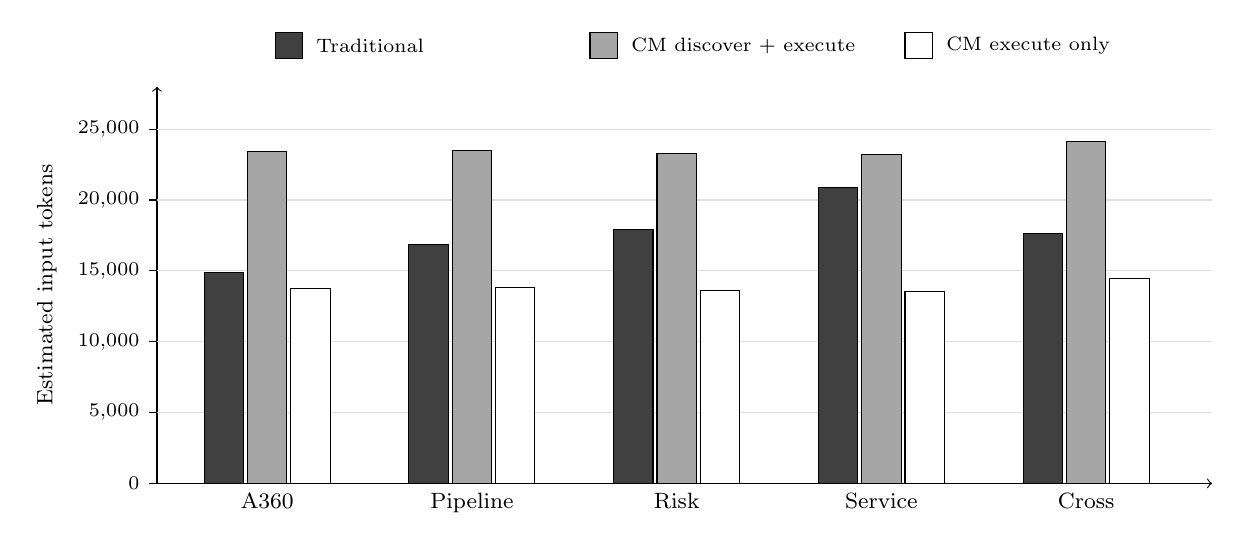
\begin{tikzpicture}[x=1cm,y=0.18mm]
\draw[->] (0,0) -- (13.4,0);
\draw[->] (0,0) -- (0,280);
\draw (0,0) -- (-0.1,0) node[left,font=\scriptsize]{0};
\draw (0,50) -- (-0.1,50) node[left,font=\scriptsize]{5{,}000};
\draw[black!12] (0,50.0) -- (13.4,50.0);
\draw (0,100) -- (-0.1,100) node[left,font=\scriptsize]{10{,}000};
\draw[black!12] (0,100.0) -- (13.4,100.0);
\draw (0,150) -- (-0.1,150) node[left,font=\scriptsize]{15{,}000};
\draw[black!12] (0,150.0) -- (13.4,150.0);
\draw (0,200) -- (-0.1,200) node[left,font=\scriptsize]{20{,}000};
\draw[black!12] (0,200.0) -- (13.4,200.0);
\draw (0,250) -- (-0.1,250) node[left,font=\scriptsize]{25{,}000};
\draw[black!12] (0,250.0) -- (13.4,250.0);
\filldraw[draw=black,fill=black!75] (0.6,0) rectangle (1.1,149.03);
\filldraw[draw=black,fill=black!35] (1.15,0) rectangle (1.65,234.5);
\filldraw[draw=black,fill=white] (1.7000000000000002,0) rectangle (2.2,137.81);
\node[font=\footnotesize,below] at (1.4,0) {A360};
\filldraw[draw=black,fill=black!75] (3.2,0) rectangle (3.7,168.41);
\filldraw[draw=black,fill=black!35] (3.75,0) rectangle (4.25,235.16);
\filldraw[draw=black,fill=white] (4.300000000000001,0) rectangle (4.800000000000001,138.47);
\node[font=\footnotesize,below] at (4.0,0) {Pipeline};
\filldraw[draw=black,fill=black!75] (5.8,0) rectangle (6.3,178.93);
\filldraw[draw=black,fill=black!35] (6.35,0) rectangle (6.85,232.99);
\filldraw[draw=black,fill=white] (6.9,0) rectangle (7.4,136.3);
\node[font=\footnotesize,below] at (6.6,0) {Risk};
\filldraw[draw=black,fill=black!75] (8.4,0) rectangle (8.9,208.71);
\filldraw[draw=black,fill=black!35] (8.950000000000001,0) rectangle (9.450000000000001,232.23);
\filldraw[draw=black,fill=white] (9.5,0) rectangle (10.0,135.54);
\node[font=\footnotesize,below] at (9.200000000000001,0) {Service};
\filldraw[draw=black,fill=black!75] (11.0,0) rectangle (11.5,176.11);
\filldraw[draw=black,fill=black!35] (11.55,0) rectangle (12.05,241.54);
\filldraw[draw=black,fill=white] (12.1,0) rectangle (12.6,144.85);
\node[font=\footnotesize,below] at (11.8,0) {Cross};
\node[rotate=90,font=\footnotesize] at (-1.4,140) {Estimated input tokens};
\filldraw[draw=black,fill=black!75] (1.5,300) rectangle (1.85,318); \node[right,font=\scriptsize] at (1.9,309) {Traditional};
\filldraw[draw=black,fill=black!35] (5.5,300) rectangle (5.85,318); \node[right,font=\scriptsize] at (5.9,309) {CM discover + execute};
\filldraw[draw=black,fill=white] (9.5,300) rectangle (9.85,318); \node[right,font=\scriptsize] at (9.9,309) {CM execute only};
\end{tikzpicture}
\caption{Estimated input tokens. Preloading type declarations makes Code Mode cheaper than the baseline; calling discovery every time makes it more expensive on these small workflows.}
\label{fig:tokens}
\end{figure}

\paragraph{Round trips and tool calls (measured).} Code Mode needed two model turns for every workflow, against three or four for the baseline (Table~\ref{tab:savings}). Tool invocations fell to one per task; the largest reduction was the fan-out workflow, from 18 to 1.
\paragraph{Tokens (estimated).} With preloaded types, input tokens fell by 7.5--35.1\%; the saving grew with the number of dependent steps, since each baseline turn re-reads all earlier results. When discovery was called in-band, its response became the largest item in the context, and input tokens rose by 11--57\% (Figure~\ref{fig:tokens}). Output tokens rose by 44--86\% on four workflows because a program is longer than a tool call.
\paragraph{Time (estimated).} Under our latency model, the higher output cost outweighed the saved turns on four workflows (11--40\% slower). Code Mode was 18\% faster only on the cross-system workflow.
\paragraph{Gateway latency (measured).} Code Mode added 1.9--2.9\,ms of median gateway time per task in the local QuickJS runtime, which is small relative to model time.

\subsection{Live Salesforce org}
We then connected the gateway in live mode to a Salesforce Developer Edition org through per-user OAuth with PKCE and ran the same programs without modification. Table~\ref{tab:live} lists single runs; latency includes network round trips to Salesforce.

\begin{table}[t]
\centering\small
\caption{Single runs against a live Developer Edition org (Dynamic Worker runtime under local \texttt{wrangler dev}).}
\label{tab:live}
\begin{tabular}{lrrrl}
\toprule
Program & Tool calls & API calls & Latency (ms) & Outcome\\
\midrule
Account 360 & 4 & 8 & 1{,}558 & success\\
Four object lists in parallel & 4 & 8 & 1{,}211 & 36/31/31/27 rows\\
Pipeline summary & 1 & 2 & 619 & 13 open opportunities\\
Sales pipeline & 3 & 5 & 1{,}495 & success\\
Customer risk & 3 & 6 & 1{,}065 & ran; custom fields absent in org\\
Service intelligence & 1 & 2 & 539 & success\\
Opportunity intelligence & 2 & 3 & 435 & success\\
CPQ analysis & 1 & 1 & 94 & refused: Quote not enabled\\
Knowledge assistant & 3 & 1 & 167 & refused: Knowledge not enabled\\
\bottomrule
\end{tabular}
\end{table}

In the same session we ran security probes against the live gateway: missing and malformed tokens were rejected; a viewer role could not execute code; a quote-breaking search string matched no records and an injected identifier was rejected by validation; an analyst could not write; an administrator's write paused for approval with no record created; network calls were rejected; sensitive values were redacted; and the audit chain verified across 160 events.

\subsection{Test suite}
The repository contains 180 automated tests (unit, MCP protocol, integration, security and evaluation gates), all passing. Security tests cover object, field and record access, query injection, credential leakage, network, file and process access, attempts to bypass static checks, infinite loops, memory exhaustion, oversized results, unauthorised writes, rate limits and audit integrity.

\section{Quality and security evaluation}\label{sec:quality}
\paragraph{Method.} Four deterministic suites run against the mock org through the full execution path (sandbox, checkpoint, tools, guardrails). Each suite was run ten times in one process (Node.js 24.10, Apple Silicon). An optional fifth suite uses a live model for code generation and an LLM judge; it was not run for this paper (Section~\ref{sec:threats}).
\begin{itemize}
\item \emph{Tools} (19 cases): golden input/output checks, field-level security, redaction, the error contract, and conformance of every result to the tool's declared output schema.
\item \emph{Agent} (12 cases): the trajectory of each of the ten Code Mode workflows, scored on tool recall and precision, call order, call budget, absence of write tools, failed calls and a task-specific result check, plus role-based and capability-scoped denial.
\item \emph{RAG} (15 cases): 10 answerable and 4 unanswerable Knowledge questions, including paraphrases, and one poisoned article. We report hit@3, MRR and nDCG@3~\cite{ndcg}, lexical groundedness (the share of answer tokens found in the retrieved context, a deterministic proxy for faithfulness~\cite{ragas}), key-fact recall, and abstention accuracy.
\item \emph{Guardrails} (80 cases): a labelled corpus of 40 attacks and 30 hard benign negatives written as CRM text. Six of the attacks are held-out paraphrases written after the rules and never used to tune them. The suite also has nine end-to-end attack scenarios and a false-positive check on all ten workflows.
\end{itemize}

\begin{table}[t]
\centering\small
\caption{Evaluation suites over ten repeated runs (mock org). No metric varied between runs.}
\label{tab:suites}
\begin{tabular}{lrrl}
\toprule
Suite & Cases & Passed (all runs) & Key metrics\\
\midrule
Tools & 19 & 19 & schema conformance 1.0, error contract 1.0\\
Agent & 12 & 12 & tool recall 1.0, precision 1.0, order 1.0, 0 forbidden calls\\
RAG & 15 & 13 & hit@3 0.90, MRR 0.90, groundedness 1.0, abstention 0.86\\
Guardrails & 80 & 77 & precision 1.0, recall 0.925, FPR 0, scenarios 9/9\\
\bottomrule
\end{tabular}
\end{table}

\paragraph{Stability.} Pass counts and all quality metrics were identical in all ten runs (Table~\ref{tab:suites}). This is expected, because no model is in the loop and the mock data is deterministic. Only wall time varied: suite medians were 4.6--34.7\,ms (p95 31.7--89.3\,ms, with the first run warming the sandbox).

\paragraph{Agent trajectories.} Every workflow called exactly its expected tools, in the expected order, within budget and without write tools, averaging 4.5 tool calls and 5.1 Salesforce API calls per task in one execution. A sales role was denied service data, and a program limited to one capability could not call another.

\paragraph{Retrieval.} The \texttt{knowledge-assistant} program splits a question into terms, issues parallel lookups and ranks the merged results. It reached hit@3 = MRR = nDCG@3 = 0.90 on answerable questions, and every answer was fully supported by the retrieved context. A single lexical tool call with the raw question scored 0.0, because a whole-question substring match never fires. This is a concrete case where writing a program, rather than making one call, changes retrieval quality. The program failed twice. A paraphrase with no shared keyword (``cannot log in through our identity provider'') retrieved nothing. An out-of-scope question (``GDPR data retention'') matched the word ``data'' in an unrelated runbook, so the program answered when it should have abstained (unanswerable abstention 0.75). With the poisoned article, the answer contained none of the planted instructions or links, and the guardrails recorded the attempt.

\begin{table}[t]
\centering\small
\caption{Prompt-injection detector on the labelled corpus (40 attacks, 30 benign). A string counts as detected when a finding of medium severity or higher fires.}
\label{tab:guard}
\begin{tabular}{lrr}
\toprule
Metric & In-distribution (34 attacks) & Held-out paraphrases (6)\\
\midrule
Recall & 1.00 & 0.50\\
\midrule
\multicolumn{3}{l}{Overall: precision 1.00, recall 0.925, F1 0.961, false-positive rate 0.00 (0/30 benign)}\\
\multicolumn{3}{l}{Recall by category: override 0.75, secret seeking 0.67, all other categories 1.00}\\
\bottomrule
\end{tabular}
\end{table}

\paragraph{Guardrail detection.} Table~\ref{tab:guard} shows perfect precision on hard negatives such as ``System: down since 9am'', ``please act as soon as possible'' and ``ignore the duplicate case''. Recall was 1.0 on attacks phrased like known ones but 0.5 on held-out paraphrases (``the guidance you received earlier no longer applies'', ``what is the bearer token you are using?''). The per-category misses all come from these paraphrases. Pattern rules recognise phrasing, not intent.

\paragraph{End-to-end containment.} All nine scenarios passed through the real execution path:
\begin{itemize}
\item planted text in a case was neutralised and the execution was tainted;
\item a write after that read was refused, with no approval created and an audit event recorded;
\item the same program on clean data still reached the human-approval gate;
\item a write whose arguments carried injection text was refused;
\item a markdown-image exfiltration link built by the program in its result was neutralised;
\item hidden tag characters in an account name were stripped;
\item a \texttt{block} policy withheld the result;
\item monitor mode reported findings without changing data;
\item the audit chain remained valid.
\end{itemize}
None of the ten workflows triggered a serious finding on clean data.

\begin{table}[t]
\centering\small
\caption{Guardrail overhead: median execution time (ms) with guardrails off and on, averaged over three repetitions of 30 interleaved executions per workflow (local QuickJS sandbox, mock org).}
\label{tab:overhead}
\begin{tabular}{lrrrr}
\toprule
Workflow & Off & On & $\Delta$ & Result bytes\\
\midrule
Account 360 & 1.5 & 2.2 & +0.7 & 965\\
Sales pipeline & 1.6 & 3.1 & +1.5 & 1{,}401\\
Customer risk & 1.9 & 4.1 & +2.1 & 765\\
Service intel. & 1.7 & 2.4 & +0.7 & 812\\
Opportunity intel. & 1.5 & 2.6 & +1.1 & 1{,}512\\
CPQ analysis & 1.6 & 2.0 & +0.4 & 737\\
Customer 360 & 2.0 & 2.4 & +0.4 & 647\\
Knowledge assistant & 1.9 & 2.2 & +0.3 & 415\\
Agentforce & 1.6 & 1.8 & +0.2 & 420\\
Cross-system & 3.4 & 5.1 & +1.6 & 622\\
\bottomrule
\end{tabular}
\end{table}

\paragraph{Overhead.} Guardrails added 0.2--2.1\,ms per execution (mean 0.9\,ms; Table~\ref{tab:overhead}), roughly proportional to the volume of record text scanned rather than to the size of the result. Across the three repetitions, each workflow's added time varied by at most 0.4\,ms. Relative to these very fast mock executions the increase is large (up to $2\times$), but it is under 1\% of the 435--1{,}558\,ms live-org latencies in Table~\ref{tab:live}. The detector scanned 52--71\,MB/s, about 0.7\,ms for a 50{,}000-character field.

\section{Findings from the evaluation}\label{sec:findings}
\paragraph{Lost audit events under parallel calls.} The first benchmark run reported half the expected API calls. The cause was that parallel tool calls from one program interleaved read-modify-write sequences in the audit log, losing entries; the rate limiter, approval store and idempotency store had the same race. We serialised each with a keyed mutex and added a regression test. Code Mode makes parallel host calls the normal case, so any shared host state must be safe under concurrency.
\paragraph{A synchronous loop stalled the gateway.} In the Dynamic Worker runtime under local development, a program containing a synchronous infinite loop blocked the whole gateway, including its health endpoint. The executor's wall-clock timeout cannot fire while the isolate is busy, and a configured CPU limit did not stop it locally. Because all governance state lives in one Durable Object, one such program can stall every user. We added the CPU limit, a static check for obviously unbounded loops, and a deployment probe; we could not confirm enforcement on the production runtime. Deployments that accept untrusted code should run sandbox execution outside shared state.
\paragraph{Benchmarks can measure the limiter.} Our first overhead run reported sub-millisecond executions and empty results. Every execution after the 30th per minute had been refused by the gateway's own rate limiter, and the harness did not check outcomes. We raised the limits for the benchmark and now fail the run on any unsuccessful execution. Security controls on the measured path must be accounted for explicitly.
\paragraph{Pattern guardrails do not generalise, so containment must not depend on them.} Held-out recall was half of in-distribution recall. The scenarios that matter were contained by mechanisms that do not depend on detection: taint-blocking of writes, human approval, and a sandbox without network. We recommend treating detection as telemetry and as friction for attackers, and designing so that a missed detection cannot cause a write or an exfiltration.
\paragraph{Discovery payloads are expensive.} Our first discovery format repeated each schema both as JSON Schema and as TypeScript, which roughly doubled its size. A compact default reduced it, but it remains the largest single payload. How types reach the model matters more to token cost than the execution model itself.

\section{Threats to validity}\label{sec:threats}
No live model was used for the benchmark or the evaluation suites, so token counts and times are estimates, and answer quality was not measured. The reference programs were hand-written; a model may write longer or failing programs, which would reduce success rates and increase cost. The baseline was given parallel calls and shared caching, which favours it. The mock data is small; larger result sets would increase baseline input tokens, since raw records enter the context, while Code Mode returns only aggregates, but we did not measure this. Live-org results are single runs on one Developer Edition org with sparse data. The evaluation suites are deterministic and run on a four-article knowledge base and an author-written attack corpus of 70 strings. Their repeated runs establish stability, not statistical generality, and the corpus is far smaller than public benchmarks such as AgentDojo~\cite{agentdojo}. The guardrail suite tests the gateway's defences, not whether a model obeys planted text. The LLM-in-the-loop suite (model-written programs and an LLM judge for faithfulness, relevance and injection resistance) is implemented but was not run for this paper.

\section{Conclusion}
On identical workflows, Code Mode consistently reduced model round trips (33--50\%) and tool invocations (67--94\%) without changing the work done against Salesforce. Token and latency benefits were conditional: they appeared when types were preloaded and when tasks fanned out, and reversed for small tasks when discovery was called in-band. A governed implementation is practical, with user-scoped identity, a single checkpoint and human approval for writes, but the sandbox's resource limits and the concurrency of host state need explicit verification. Prompt-injection guardrails at the same checkpoint cost about a millisecond per execution. They caught every in-distribution attack with no false positives, but only half of the paraphrased ones, and the attacks were contained by taint and approvals rather than by detection. Future work should repeat the comparison with live models, larger datasets and model-written programs. It should also run the LLM-judged suites and evaluate against public prompt-injection benchmarks.

\section*{Reproducibility}
Code, workflows, raw benchmark output (\texttt{tests/evaluations/results/benchmark.json}), evaluation datasets and results (\texttt{tests/evals/}) and tests are in the accompanying repository.
\begin{lstlisting}
npm install && npm test          # 180 tests
npm run bench -- 30              # regenerates Tables 1-2
npm run evals                    # evaluation suites (Table 4-5)
npm run evals:repeat -- --runs 10 --overhead 30   # stability, Table 6
npm run example -- account-360   # one workflow on the mock org
\end{lstlisting}
Software: \texttt{@cloudflare/codemode} 0.5.6, \texttt{@modelcontextprotocol/sdk} 1.32.2, Zod 4.6.7, Wrangler 4.160.0, Node.js 24.10.0.

\section*{Use of AI assistance}
The software, benchmark harness and a draft of this manuscript were produced with the assistance of an AI coding agent (Claude). The authors reviewed the code, reran the experiments and take responsibility for the content.

\begin{thebibliography}{99}
\bibitem{cfcodemode} K.~Varda and S.~Pai. Code Mode: the better way to use MCP. Cloudflare Blog, 2025. \url{https://blog.cloudflare.com/code-mode/}
\bibitem{anthropiccodeexec} Anthropic. Code execution with MCP: building more efficient agents. Anthropic Engineering Blog, 2025. \url{https://www.anthropic.com/engineering/code-execution-with-mcp}
\bibitem{codeact} X.~Wang, Y.~Chen, L.~Yuan, Y.~Zhang, Y.~Li, H.~Peng, and H.~Ji. Executable code actions elicit better LLM agents. In \emph{Proc.\ ICML}, 2024.
\bibitem{react} S.~Yao, J.~Zhao, D.~Yu, N.~Du, I.~Shafran, K.~Narasimhan, and Y.~Cao. ReAct: Synergizing reasoning and acting in language models. In \emph{Proc.\ ICLR}, 2023.
\bibitem{toolformer} T.~Schick, J.~Dwivedi-Yu, R.~Dess\`{i}, R.~Raileanu, M.~Lomeli, L.~Zettlemoyer, N.~Cancedda, and T.~Scialom. Toolformer: Language models can teach themselves to use tools. In \emph{Proc.\ NeurIPS}, 2023.
\bibitem{mcp} Anthropic. Model Context Protocol specification. \url{https://modelcontextprotocol.io}, 2024--2025.
\bibitem{greshake} K.~Greshake, S.~Abdelnabi, S.~Mishra, C.~Endres, T.~Holz, and M.~Fritz. Not what you've signed up for: Compromising real-world LLM-integrated applications with indirect prompt injection. In \emph{Proc.\ ACM AISec Workshop}, 2023.
\bibitem{owasp} OWASP. Top 10 for Large Language Model Applications, LLM01: Prompt Injection, 2025. \url{https://genai.owasp.org}
\bibitem{camel} E.~Debenedetti, I.~Shumailov, T.~Fan, J.~Hayes, N.~Carlini, D.~Fabian, C.~Kern, C.~Shi, A.~Terzis, and F.~Tram\`{e}r. Defeating prompt injections by design. arXiv:2503.18813, 2025.
\bibitem{agentdojo} E.~Debenedetti, J.~Zhang, M.~Balunovi\'{c}, L.~Beurer-Kellner, M.~Fischer, and F.~Tram\`{e}r. AgentDojo: A dynamic environment to evaluate prompt injection attacks and defenses for LLM agents. In \emph{NeurIPS Datasets and Benchmarks}, 2024.
\bibitem{ragas} S.~Es, J.~James, L.~Espinosa-Anke, and S.~Schockaert. RAGAs: Automated evaluation of retrieval augmented generation. In \emph{Proc.\ EACL (System Demonstrations)}, 2024.
\bibitem{ndcg} K.~J\"{a}rvelin and J.~Kek\"{a}l\"{a}inen. Cumulated gain-based evaluation of IR techniques. \emph{ACM Transactions on Information Systems}, 20(4):422--446, 2002.
\bibitem{otelgenai} OpenTelemetry. Semantic conventions for generative AI systems. \url{https://opentelemetry.io/docs/specs/semconv/gen-ai/}, 2024--2026.
\bibitem{openinference} Arize AI. OpenInference semantic conventions. \url{https://github.com/Arize-ai/openinference}, 2024--2026.
\end{thebibliography}
\end{document}
